%----------------------------------------------------------------------------------------
%
%   LP-SZ
%
%----------------------------------------------------------------------------------------
%\chapter{Le programme cosmologique de NIKA2}

{\color{vert}\lipsum[4]}

%  VOIR PROCEEDIND MORIOND 2018 :
%/Users/perotto/MesTrucs/Talks/proceedings/Moriond-2018
%--------------------------------------------------------
\section{Observer à haute résolution angulaire}

% 1 page
\subsection{Motivation pour la cosmologie}
{\color{vert}\lipsum[2-4]}
\subsection{\'Etudes pilotes avec le prototype NIKA}
{\color{vert}\lipsum[5-7]}

\section{Le grand programme d'observation d'amas de galaxies}

% 1 page
{\color{vert}\lipsum[2-5]}

\begin{figure}
  \centering
  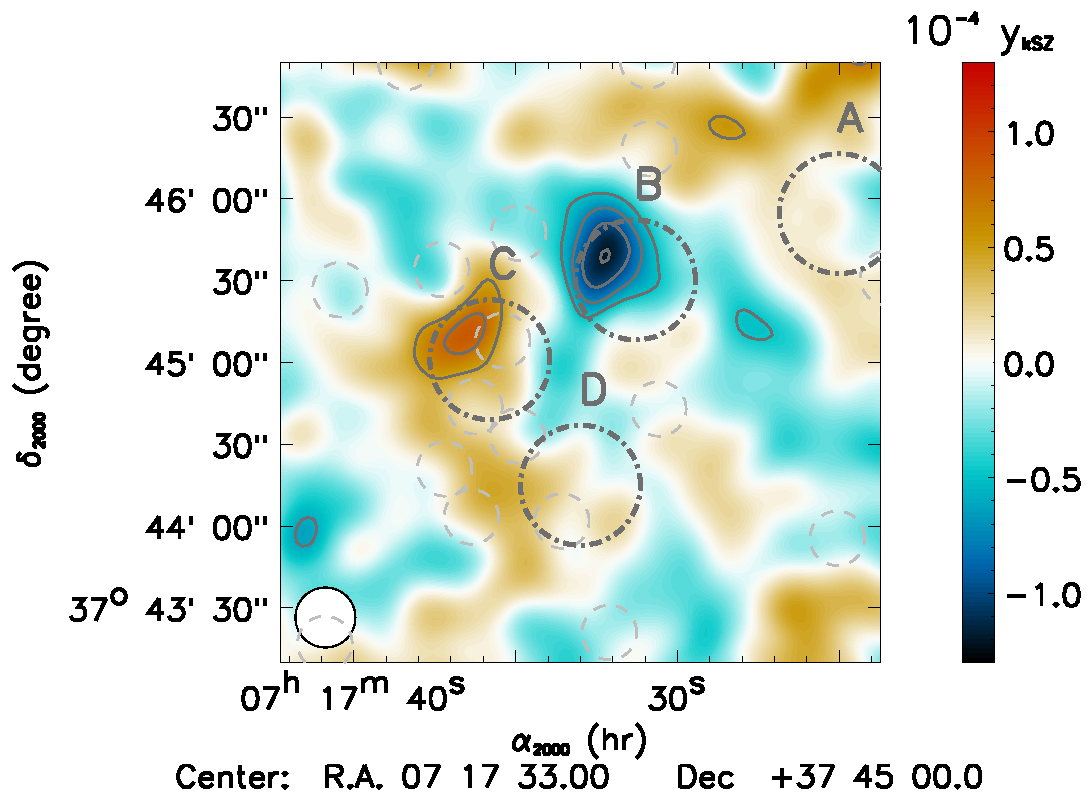
\includegraphics[width=0.49\textwidth]{Figures/NIKA2-SZ/MACSJ0717_kSZ_map.pdf}
  \hspace{4mm}
  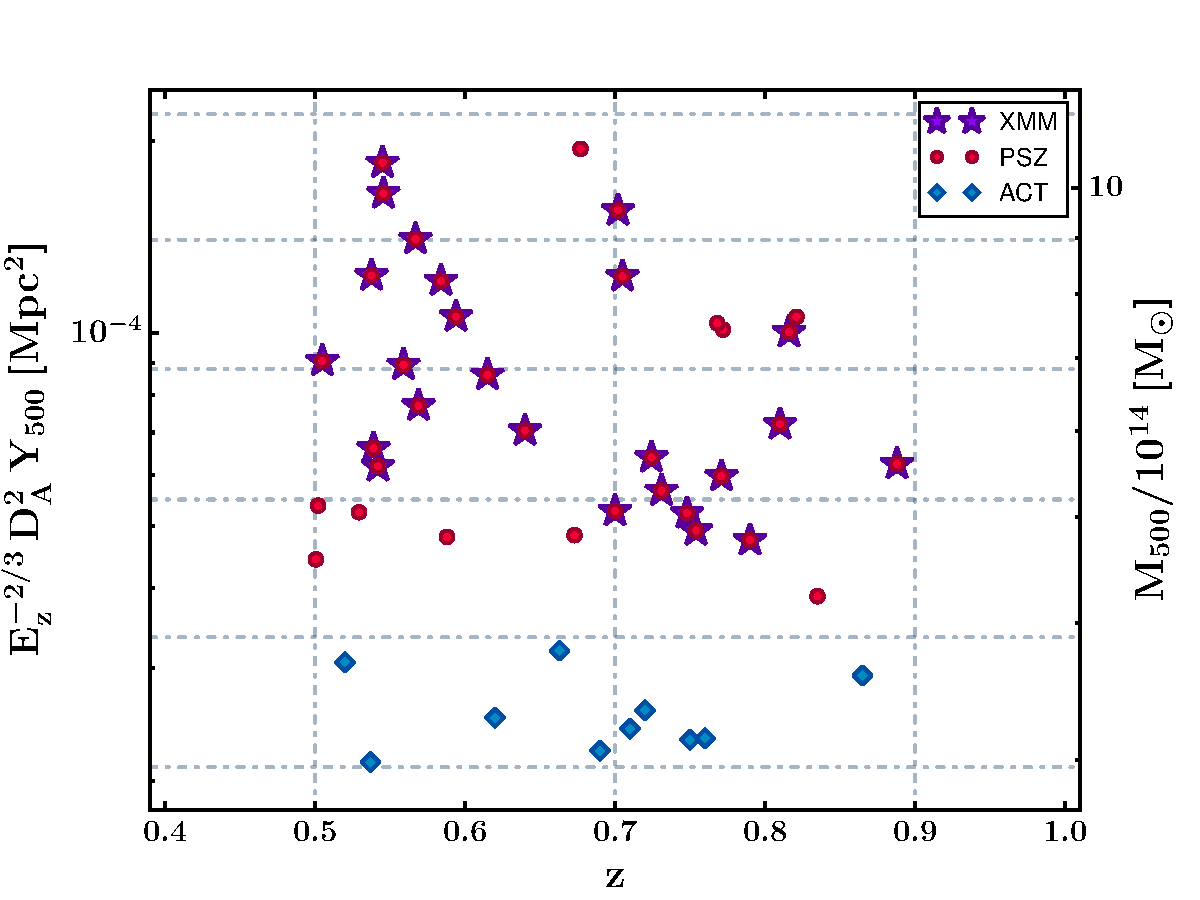
\includegraphics[width=0.44\textwidth, clip=true, trim=0cm -0.7cm 0cm 0cm]{Figures/NIKA2-SZ/LPSZ_M_z_grid.pdf}
  \caption{Left: Map of the kinetic SZ effect toward \mbox{MACS~J0717.5+3745} using NIKA pathfinder data, as discussed in Adam et al. (2017)$^{31}$. Right: NIKA2 Guaranteed-time cosmology program sample of galaxy clusters}
  \label{fig:nikanika2}
\end{figure}

\section{Premiers résultats et perspectives}

% 2 page
{\color{vert}\lipsum[2-5]}

\begin{figure}
  \centering
  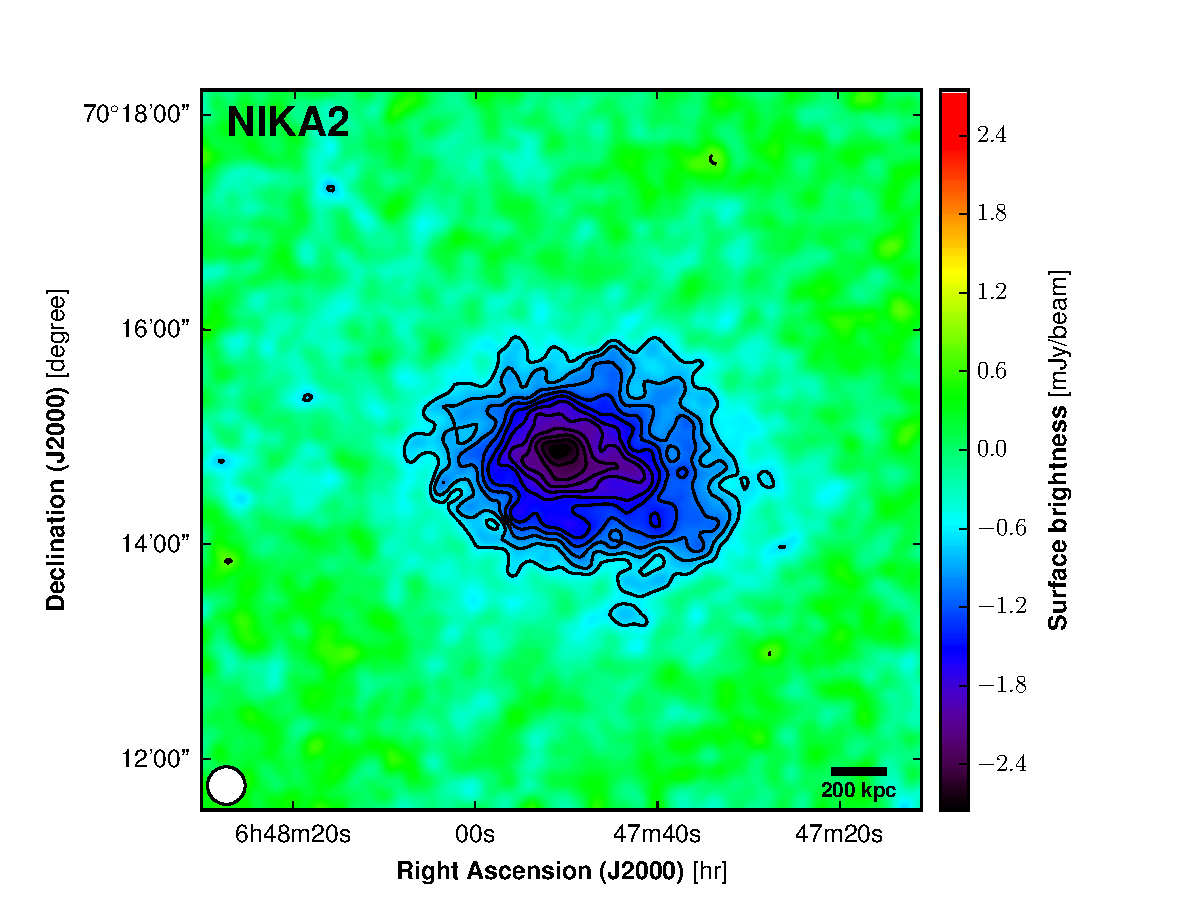
\includegraphics[width=0.49\textwidth]{Figures/NIKA2-SZ/Paper_NIKA2_Data.pdf}
  \includegraphics[width=0.44\textwidth]{Figures/NIKA2-SZ/Fig_PSZ2_G144_Scaling_relation.pdf}
  \caption{First SZ results with NIKA2. Left: The NIKA2 SZ map toward the galaxy cluster PSZ2-G0144.83+25.11. The high-resolution (20~arcsec) high-accuracy ($13.5\sigma $ measurement at peak) map covers the cluster from the core to the outskirts and reveals its morphology. An excess SZ signal is observed in the South-West region, indicating an overpressure within the intracluster medium (ICM). Right: Illustration of the impact of the ICM dynamics on the inner scatter of the SZ mass-observable relation. NIKA2 $Y_{500}$ estimates from the analysis with and without masking the over-pressure of PSZ2-G0144.83+25.11 are shown as a function of $M_{500}$, along with the cluster sample and the $Y_{500}-M_{500}$ scaling relation used in \emph{Planck} SZ-selected cluster count based cosmology analysis$^{13}$. These figures are extracted from Ruppin {\it et al.} (2018)$^{34}$. }
  \label{fig:nika2-sz}
\end{figure}

{\color{vert}\lipsum[2-5]}
